\subsection{The Top-level Abstract Model}
\label{sec:component_diagrams-tutorial_topLevelAbstractModel}


The modelling process begins by describing a single, abstract state machine that represents the washing machine together with its environment. Four states represent the modes of the system: IDLE, WASHING, RINSING and SPINNING and seven transitions represent how the system modes evolve. A component WM is also introduced to represent the complete system. It contains the state-machine and owns operations that link to the transitions in the state-machine. The top-level component and state machine are shown in Figure \ref{fig:AbstractModelOfAWashingMachine}.
At this stage the transition operations in the component WM add little to the model but they are needed due to a limitation (explained below) of the representation of self-wake events. Since self-wake events are modelled in Event-B by a single generated variable per component, any operations of a component that, in future refinements, alter the state of self-wakes must be added when the component is first introduced. If they were added later the rules of refinement would prevent them from altering the self-wake variable.

 \begin{figure}[!htbp]
  \centering
  \ifplastex
  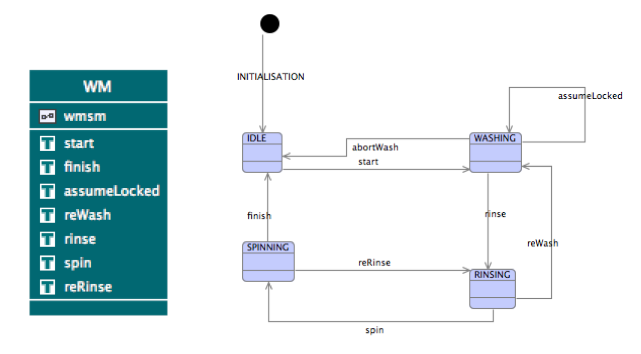
\includegraphics[width=1024]{figures/image13.png}
  \else
  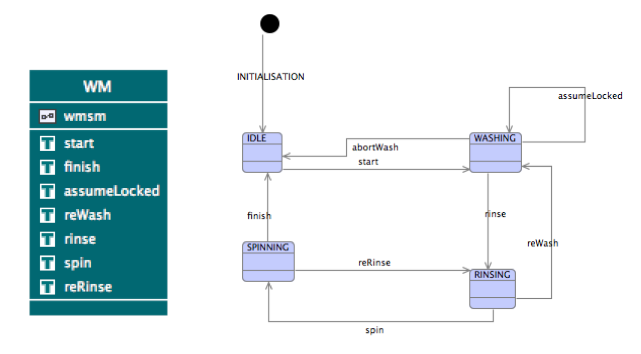
\includegraphics[width=1\textwidth]{figures/image13.png}
  \fi
  \caption{Abstract Model of a Washing Machine}
  \label{fig:AbstractModelOfAWashingMachine}
\end{figure} 

This system-level state machine is untimed and non-deterministic. For instance, when the system is in state RINSING, the system will immediately move to either state SPINNING or WASHING non-deterministically. The state machine represents all the possible mode traces of the system.
Once the state machine has been constructed, the first step is to ensure that all the proof obligations that have been generated by the CODA tool are discharged successfully, as shown in Figure \ref{fig:DischargedProofObligationsOfTheAbstractModel} below. Usually, if the user has added no extra invariants to the model, all the proof obligations should be discharged automatically. If any proof obligations have not been discharged (indicated by an orange question mark icon) they should be examined to determine whether there is a problem with the model. To examine a proof obligation, double click on its icon in the navigator. Switch to the proving perspective by clicking the green tick icon in the right hand corner of the menu bar.  Examine the goal as well as the information tab to work out what the prover is attempting to prove.
 
 \begin{figure}[!htbp]
  \centering
  \ifplastex
  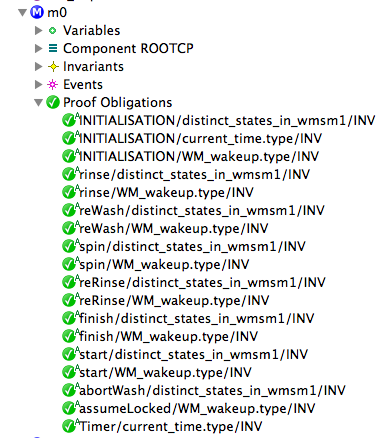
\includegraphics[width=1024]{figures/image14.png}
  \else
  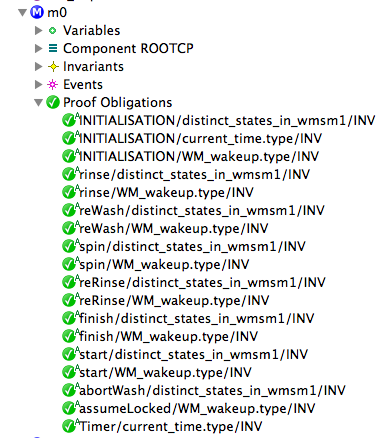
\includegraphics[width=1\textwidth]{figures/image14.png}
  \fi
  \caption{Discharged Proof Obligations of the Abstract Model}
  \label{fig:DischargedProofObligationsOfTheAbstractModel}
\end{figure} 

The next step in the process is to animate the system-level state machine to validate that states and transitions correctly represent the system-level view of the washing machine as shown in Figure \ref{fig:AnimatingTheStatemachineOfTheAbstractModel}. This is a validation process requiring subjective evaluation of the model against system requirements. Does the state-machine behave as desired?

 \begin{figure}[!htbp]
  \centering
  \ifplastex
  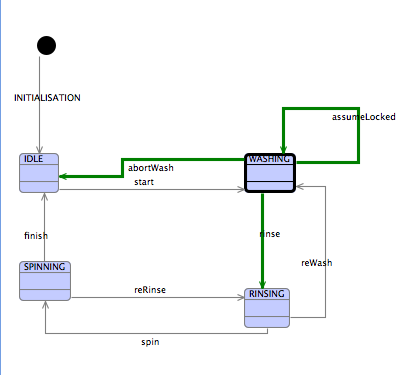
\includegraphics[width=1024]{figures/image15.png}
  \else
  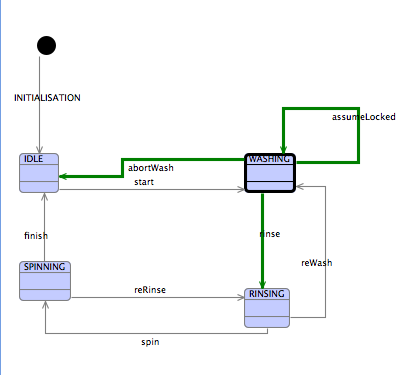
\includegraphics[width=1\textwidth]{figures/image15.png}
  \fi
  \caption{Animating the State-machine of the Abstract Model}
  \label{fig:AnimatingTheStatemachineOfTheAbstractModel}
\end{figure} 

The current state of the system is WASHING, as indicated by the bold, black outline of the state. Three transitions, highlighted in green, are enabled from this state: abortWash, rinse and assumeLocked. Select one from this non-deterministic choice to proceed with the animation. Continue animating the state machine to validate this top-level specification against the system requirements.
The specification may also be validated from the ProB view of Rodin as shown in Figure \ref{fig:AnimatingTheAbstractModelWithProBEventAndHistoryViews} and Figure \ref{fig:AnimatingTheAbstractModelWithProBStateView} below. The event view of Figure  \ref{fig:AnimatingTheAbstractModelWithProBEventAndHistoryViews} presents a list of enabled events from which one may be selected to advance the animation. The history view of Figure  \ref{fig:AnimatingTheAbstractModelWithProBEventAndHistoryViews} shows a record of previous selections. At any stage of the animation it is possible to go back to a selection in the history and perform a new animation from that point.
 
 \begin{figure}[!htbp]
  \centering
  \ifplastex
  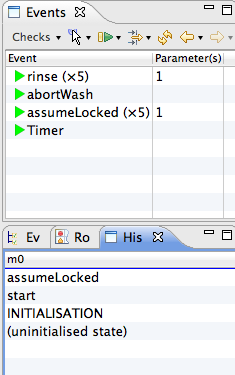
\includegraphics[width=1024]{figures/image16.png}
  \else
  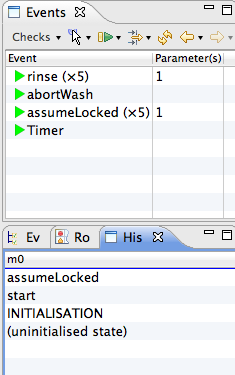
\includegraphics[width=1\textwidth]{figures/image16.png}
  \fi
  \caption{Animating the Abstract Model with ProB Event and History Views}
  \label{fig:AnimatingTheAbstractModelWithProBEventAndHistoryViews}
\end{figure} 

The state view of Figure \ref{fig:AnimatingTheAbstractModelWithProBStateView} shows the current and previous value for each variable. The invariants and guards may also be analysed in this view. The final verification step is to show absence of deadlock using the ProB model checker.

 \begin{figure}[!htbp]
  \centering
  \ifplastex
  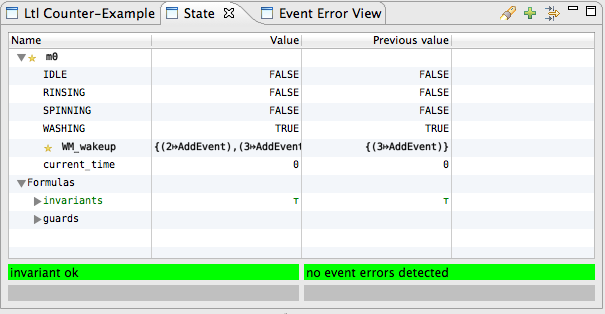
\includegraphics[width=1024]{figures/image17.png}
  \else
  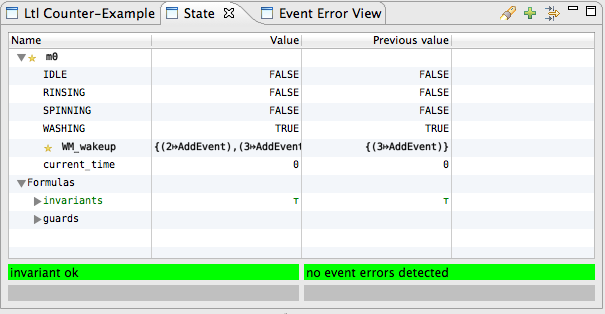
\includegraphics[width=1\textwidth]{figures/image17.png}
  \fi
  \caption{Animating the Abstract Model with ProB State View}
  \label{fig:AnimatingTheAbstractModelWithProBStateView}
\end{figure} 

First the model checker is configured as shown in Figure \ref{fig:ProBModelCheckerOptions} to find deadlocks and invariant violations. For this abstract model, the automatic provers have already proved all the proof obligations, but later in the refinement process it may be more difficult to prove some of the invariants. The model checker can then be used to look for counterexamples that are due to modelling errors. If the model checker reveals a counterexample it is more efficient than embarking on a complex proof that is eventually found to be false. If a counterexample is not revealed (and the complete state space has not been covered) the goal of the proof may still be false. Therefore the goals to be proven should be examined carefully as they often reveal a problem with the model. 
It is important not to leave unproven invariants in a model since if they are not true these could be used in later refinements by the automatic provers to make incorrect deductions.
Selecting symmetry reduction option is not really necessary at this stage, but can help to reduce model checking time when the model is more complex.
When the model checking completes, the results are presented by ProB in the window shown in Figure \ref{fig:ProBModelCheckingCoverageForTheAbstractModel} below.
 
 \begin{figure}[!htbp]
  \centering
  \ifplastex
  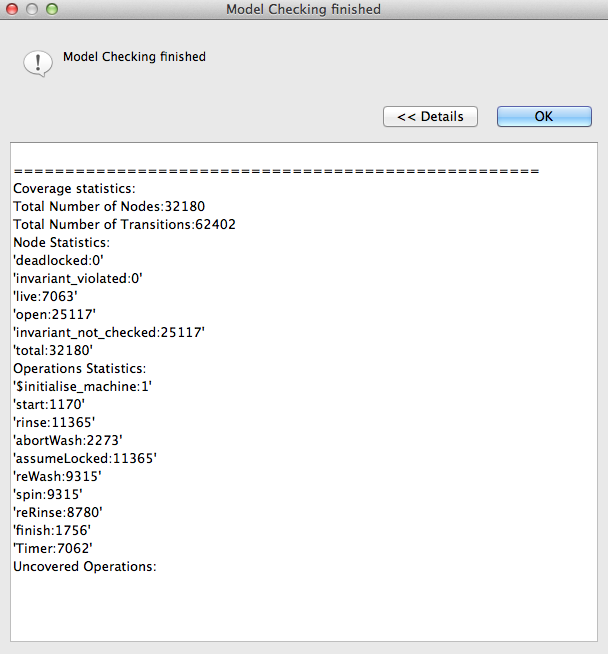
\includegraphics[width=1024]{figures/image18.png}
  \else
  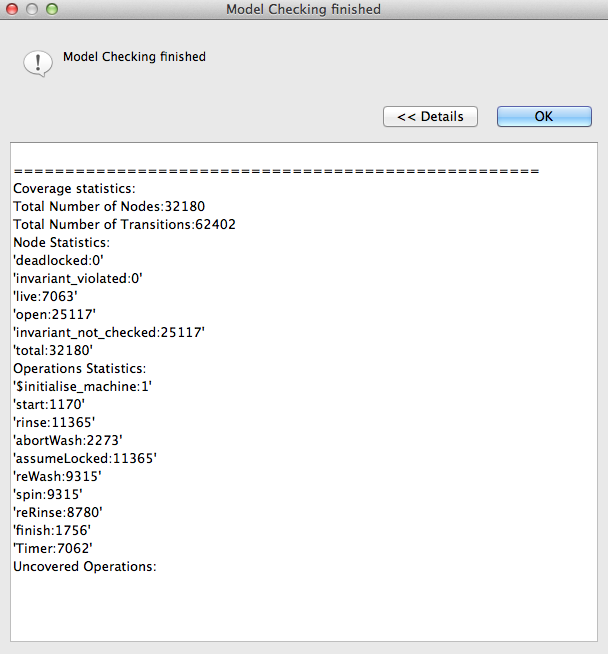
\includegraphics[width=1\textwidth]{figures/image18.png}
  \fi
  \caption{ProB Model Checking Coverage for the Abstract Model}
  \label{fig:ProBModelCheckingCoverageForTheAbstractModel}
\end{figure} 

The interesting coverage metric is shown at the bottom of the window: Uncovered Operations. In this case all operations have been covered which increases confidence in the absence of deadlock.

%%% Local Variables:
%%% mode: latex
%%% TeX-master: "component_diagrams-user_manual"
%%% End:
